% Graphic for TeX using PGF
% Title: E:\workspace\go\src\github.com\bachopp\thesis\files\chapters\implementation\graphics\storedep.dia
% Creator: Dia v0.97.2
% CreationDate: Wed May 18 02:14:45 2016
% For: Tomasz
% \usepackage{tikz}
% The following commands are not supported in PSTricks at present
% We define them conditionally, so when they are implemented,
% this pgf file will use them.
\ifx\du\undefined
  \newlength{\du}
\fi
\setlength{\du}{15\unitlength}
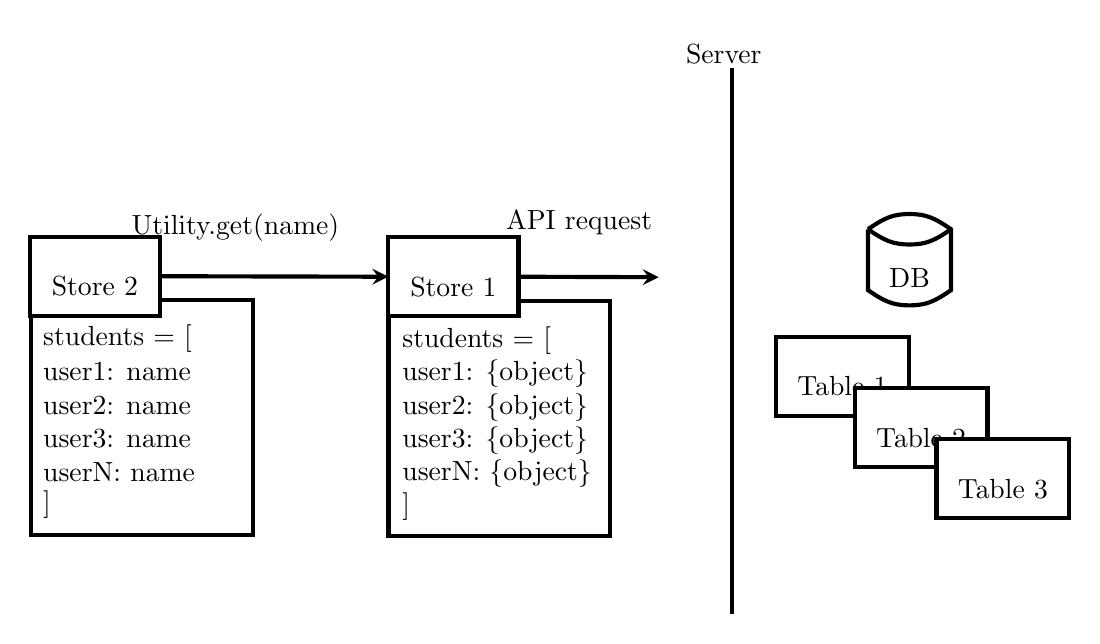
\begin{tikzpicture}
\pgftransformxscale{1.000000}
\pgftransformyscale{-1.000000}
\definecolor{dialinecolor}{rgb}{0.000000, 0.000000, 0.000000}
\pgfsetstrokecolor{dialinecolor}
\definecolor{dialinecolor}{rgb}{1.000000, 1.000000, 1.000000}
\pgfsetfillcolor{dialinecolor}
% setfont left to latex
\definecolor{dialinecolor}{rgb}{0.000000, 0.000000, 0.000000}
\pgfsetstrokecolor{dialinecolor}
\node[anchor=west] at (22.766503\du,7.489415\du){};
\definecolor{dialinecolor}{rgb}{1.000000, 1.000000, 1.000000}
\pgfsetfillcolor{dialinecolor}
\fill (13.125518\du,8.118742\du)--(13.125518\du,13.775870\du)--(18.468959\du,13.775870\du)--(18.468959\du,8.118742\du)--cycle;
\pgfsetlinewidth{0.100000\du}
\pgfsetdash{}{0pt}
\pgfsetdash{}{0pt}
\pgfsetmiterjoin
\definecolor{dialinecolor}{rgb}{0.000000, 0.000000, 0.000000}
\pgfsetstrokecolor{dialinecolor}
\draw (13.125518\du,8.118742\du)--(13.125518\du,13.775870\du)--(18.468959\du,13.775870\du)--(18.468959\du,8.118742\du)--cycle;
% setfont left to latex
\definecolor{dialinecolor}{rgb}{0.000000, 0.000000, 0.000000}
\pgfsetstrokecolor{dialinecolor}
\node at (15.797239\du,11.187306\du){};
\definecolor{dialinecolor}{rgb}{1.000000, 1.000000, 1.000000}
\pgfsetfillcolor{dialinecolor}
\fill (4.516964\du,8.089850\du)--(4.516964\du,13.746979\du)--(9.860404\du,13.746979\du)--(9.860404\du,8.089850\du)--cycle;
\pgfsetlinewidth{0.100000\du}
\pgfsetdash{}{0pt}
\pgfsetdash{}{0pt}
\pgfsetmiterjoin
\definecolor{dialinecolor}{rgb}{0.000000, 0.000000, 0.000000}
\pgfsetstrokecolor{dialinecolor}
\draw (4.516964\du,8.089850\du)--(4.516964\du,13.746979\du)--(9.860404\du,13.746979\du)--(9.860404\du,8.089850\du)--cycle;
% setfont left to latex
\definecolor{dialinecolor}{rgb}{0.000000, 0.000000, 0.000000}
\pgfsetstrokecolor{dialinecolor}
\node at (7.188684\du,11.158415\du){};
\pgfsetlinewidth{0.100000\du}
\pgfsetdash{}{0pt}
\pgfsetdash{}{0pt}
\pgfsetbuttcap
\pgfsetmiterjoin
\pgfsetlinewidth{0.100000\du}
\pgfsetbuttcap
\pgfsetmiterjoin
\pgfsetdash{}{0pt}
\definecolor{dialinecolor}{rgb}{1.000000, 1.000000, 1.000000}
\pgfsetfillcolor{dialinecolor}
\pgfpathmoveto{\pgfpoint{24.676783\du}{6.391692\du}}
\pgfpathcurveto{\pgfpoint{25.076783\du}{6.116692\du}}{\pgfpoint{25.276783\du}{6.025026\du}}{\pgfpoint{25.676783\du}{6.025026\du}}
\pgfpathcurveto{\pgfpoint{26.076783\du}{6.025026\du}}{\pgfpoint{26.276783\du}{6.116692\du}}{\pgfpoint{26.676783\du}{6.391692\du}}
\pgfpathlineto{\pgfpoint{26.676783\du}{7.858359\du}}
\pgfpathcurveto{\pgfpoint{26.276783\du}{8.133359\du}}{\pgfpoint{26.076783\du}{8.225026\du}}{\pgfpoint{25.676783\du}{8.225026\du}}
\pgfpathcurveto{\pgfpoint{25.276783\du}{8.225026\du}}{\pgfpoint{25.076783\du}{8.133359\du}}{\pgfpoint{24.676783\du}{7.858359\du}}
\pgfpathlineto{\pgfpoint{24.676783\du}{6.391692\du}}
\pgfusepath{fill}
\definecolor{dialinecolor}{rgb}{0.000000, 0.000000, 0.000000}
\pgfsetstrokecolor{dialinecolor}
\pgfpathmoveto{\pgfpoint{24.676783\du}{6.391692\du}}
\pgfpathcurveto{\pgfpoint{25.076783\du}{6.116692\du}}{\pgfpoint{25.276783\du}{6.025026\du}}{\pgfpoint{25.676783\du}{6.025026\du}}
\pgfpathcurveto{\pgfpoint{26.076783\du}{6.025026\du}}{\pgfpoint{26.276783\du}{6.116692\du}}{\pgfpoint{26.676783\du}{6.391692\du}}
\pgfpathlineto{\pgfpoint{26.676783\du}{7.858359\du}}
\pgfpathcurveto{\pgfpoint{26.276783\du}{8.133359\du}}{\pgfpoint{26.076783\du}{8.225026\du}}{\pgfpoint{25.676783\du}{8.225026\du}}
\pgfpathcurveto{\pgfpoint{25.276783\du}{8.225026\du}}{\pgfpoint{25.076783\du}{8.133359\du}}{\pgfpoint{24.676783\du}{7.858359\du}}
\pgfpathlineto{\pgfpoint{24.676783\du}{6.391692\du}}
\pgfusepath{stroke}
\pgfsetbuttcap
\pgfsetmiterjoin
\pgfsetdash{}{0pt}
\definecolor{dialinecolor}{rgb}{0.000000, 0.000000, 0.000000}
\pgfsetstrokecolor{dialinecolor}
\pgfpathmoveto{\pgfpoint{24.676783\du}{6.391692\du}}
\pgfpathcurveto{\pgfpoint{25.076783\du}{6.666692\du}}{\pgfpoint{25.276783\du}{6.758359\du}}{\pgfpoint{25.676783\du}{6.758359\du}}
\pgfpathcurveto{\pgfpoint{26.076783\du}{6.758359\du}}{\pgfpoint{26.276783\du}{6.666692\du}}{\pgfpoint{26.676783\du}{6.391692\du}}
\pgfusepath{stroke}
% setfont left to latex
\definecolor{dialinecolor}{rgb}{0.000000, 0.000000, 0.000000}
\pgfsetstrokecolor{dialinecolor}
\node at (25.676783\du,7.558359\du){DB};
\definecolor{dialinecolor}{rgb}{1.000000, 1.000000, 1.000000}
\pgfsetfillcolor{dialinecolor}
\fill (22.461754\du,8.983490\du)--(22.461754\du,10.883490\du)--(25.661754\du,10.883490\du)--(25.661754\du,8.983490\du)--cycle;
\pgfsetlinewidth{0.100000\du}
\pgfsetdash{}{0pt}
\pgfsetdash{}{0pt}
\pgfsetmiterjoin
\definecolor{dialinecolor}{rgb}{0.000000, 0.000000, 0.000000}
\pgfsetstrokecolor{dialinecolor}
\draw (22.461754\du,8.983490\du)--(22.461754\du,10.883490\du)--(25.661754\du,10.883490\du)--(25.661754\du,8.983490\du)--cycle;
% setfont left to latex
\definecolor{dialinecolor}{rgb}{0.000000, 0.000000, 0.000000}
\pgfsetstrokecolor{dialinecolor}
\node at (24.061754\du,10.173490\du){Table 1};
\definecolor{dialinecolor}{rgb}{1.000000, 1.000000, 1.000000}
\pgfsetfillcolor{dialinecolor}
\fill (24.355564\du,10.220264\du)--(24.355564\du,12.120264\du)--(27.555564\du,12.120264\du)--(27.555564\du,10.220264\du)--cycle;
\pgfsetlinewidth{0.100000\du}
\pgfsetdash{}{0pt}
\pgfsetdash{}{0pt}
\pgfsetmiterjoin
\definecolor{dialinecolor}{rgb}{0.000000, 0.000000, 0.000000}
\pgfsetstrokecolor{dialinecolor}
\draw (24.355564\du,10.220264\du)--(24.355564\du,12.120264\du)--(27.555564\du,12.120264\du)--(27.555564\du,10.220264\du)--cycle;
% setfont left to latex
\definecolor{dialinecolor}{rgb}{0.000000, 0.000000, 0.000000}
\pgfsetstrokecolor{dialinecolor}
\node at (25.955564\du,11.410264\du){Table 2};
\definecolor{dialinecolor}{rgb}{1.000000, 1.000000, 1.000000}
\pgfsetfillcolor{dialinecolor}
\fill (26.326672\du,11.451091\du)--(26.326672\du,13.351091\du)--(29.526672\du,13.351091\du)--(29.526672\du,11.451091\du)--cycle;
\pgfsetlinewidth{0.100000\du}
\pgfsetdash{}{0pt}
\pgfsetdash{}{0pt}
\pgfsetmiterjoin
\definecolor{dialinecolor}{rgb}{0.000000, 0.000000, 0.000000}
\pgfsetstrokecolor{dialinecolor}
\draw (26.326672\du,11.451091\du)--(26.326672\du,13.351091\du)--(29.526672\du,13.351091\du)--(29.526672\du,11.451091\du)--cycle;
% setfont left to latex
\definecolor{dialinecolor}{rgb}{0.000000, 0.000000, 0.000000}
\pgfsetstrokecolor{dialinecolor}
\node at (27.926672\du,12.641091\du){Table 3};
\definecolor{dialinecolor}{rgb}{1.000000, 1.000000, 1.000000}
\pgfsetfillcolor{dialinecolor}
\fill (4.483682\du,6.573025\du)--(4.483682\du,8.473025\du)--(7.621182\du,8.473025\du)--(7.621182\du,6.573025\du)--cycle;
\pgfsetlinewidth{0.100000\du}
\pgfsetdash{}{0pt}
\pgfsetdash{}{0pt}
\pgfsetmiterjoin
\definecolor{dialinecolor}{rgb}{0.000000, 0.000000, 0.000000}
\pgfsetstrokecolor{dialinecolor}
\draw (4.483682\du,6.573025\du)--(4.483682\du,8.473025\du)--(7.621182\du,8.473025\du)--(7.621182\du,6.573025\du)--cycle;
% setfont left to latex
\definecolor{dialinecolor}{rgb}{0.000000, 0.000000, 0.000000}
\pgfsetstrokecolor{dialinecolor}
\node at (6.052432\du,7.763025\du){Store 2};
\definecolor{dialinecolor}{rgb}{1.000000, 1.000000, 1.000000}
\pgfsetfillcolor{dialinecolor}
\fill (13.120646\du,6.585451\du)--(13.120646\du,8.485451\du)--(16.258146\du,8.485451\du)--(16.258146\du,6.585451\du)--cycle;
\pgfsetlinewidth{0.100000\du}
\pgfsetdash{}{0pt}
\pgfsetdash{}{0pt}
\pgfsetmiterjoin
\definecolor{dialinecolor}{rgb}{0.000000, 0.000000, 0.000000}
\pgfsetstrokecolor{dialinecolor}
\draw (13.120646\du,6.585451\du)--(13.120646\du,8.485451\du)--(16.258146\du,8.485451\du)--(16.258146\du,6.585451\du)--cycle;
% setfont left to latex
\definecolor{dialinecolor}{rgb}{0.000000, 0.000000, 0.000000}
\pgfsetstrokecolor{dialinecolor}
\node at (14.689396\du,7.775451\du){Store 1};
% setfont left to latex
\definecolor{dialinecolor}{rgb}{0.000000, 0.000000, 0.000000}
\pgfsetstrokecolor{dialinecolor}
\node[anchor=west] at (13.188622\du,9.080337\du){students = \ensuremath{[}};
% setfont left to latex
\definecolor{dialinecolor}{rgb}{0.000000, 0.000000, 0.000000}
\pgfsetstrokecolor{dialinecolor}
\node[anchor=west] at (13.188622\du,9.880337\du){user1: \{object\}};
% setfont left to latex
\definecolor{dialinecolor}{rgb}{0.000000, 0.000000, 0.000000}
\pgfsetstrokecolor{dialinecolor}
\node[anchor=west] at (13.188622\du,10.680337\du){user2: \{object\}};
% setfont left to latex
\definecolor{dialinecolor}{rgb}{0.000000, 0.000000, 0.000000}
\pgfsetstrokecolor{dialinecolor}
\node[anchor=west] at (13.188622\du,11.480337\du){user3: \{object\}};
% setfont left to latex
\definecolor{dialinecolor}{rgb}{0.000000, 0.000000, 0.000000}
\pgfsetstrokecolor{dialinecolor}
\node[anchor=west] at (13.188622\du,12.280337\du){userN: \{object\}};
% setfont left to latex
\definecolor{dialinecolor}{rgb}{0.000000, 0.000000, 0.000000}
\pgfsetstrokecolor{dialinecolor}
\node[anchor=west] at (13.188622\du,13.080337\du){\ensuremath{]}};
% setfont left to latex
\definecolor{dialinecolor}{rgb}{0.000000, 0.000000, 0.000000}
\pgfsetstrokecolor{dialinecolor}
\node[anchor=west] at (4.535644\du,9.029588\du){students = \ensuremath{[}};
% setfont left to latex
\definecolor{dialinecolor}{rgb}{0.000000, 0.000000, 0.000000}
\pgfsetstrokecolor{dialinecolor}
\node[anchor=west] at (4.535644\du,9.829588\du){user1: name};
% setfont left to latex
\definecolor{dialinecolor}{rgb}{0.000000, 0.000000, 0.000000}
\pgfsetstrokecolor{dialinecolor}
\node[anchor=west] at (4.535644\du,10.629588\du){user2: name};
% setfont left to latex
\definecolor{dialinecolor}{rgb}{0.000000, 0.000000, 0.000000}
\pgfsetstrokecolor{dialinecolor}
\node[anchor=west] at (4.535644\du,11.429588\du){user3: name};
% setfont left to latex
\definecolor{dialinecolor}{rgb}{0.000000, 0.000000, 0.000000}
\pgfsetstrokecolor{dialinecolor}
\node[anchor=west] at (4.535644\du,12.229588\du){userN: name};
% setfont left to latex
\definecolor{dialinecolor}{rgb}{0.000000, 0.000000, 0.000000}
\pgfsetstrokecolor{dialinecolor}
\node[anchor=west] at (4.535644\du,13.029588\du){\ensuremath{]}};
\pgfsetlinewidth{0.100000\du}
\pgfsetdash{}{0pt}
\pgfsetdash{}{0pt}
\pgfsetbuttcap
{
\definecolor{dialinecolor}{rgb}{0.000000, 0.000000, 0.000000}
\pgfsetfillcolor{dialinecolor}
% was here!!!
\pgfsetarrowsend{stealth}
\definecolor{dialinecolor}{rgb}{0.000000, 0.000000, 0.000000}
\pgfsetstrokecolor{dialinecolor}
\draw (7.621182\du,7.523025\du)--(13.120646\du,7.535451\du);
}
\pgfsetlinewidth{0.100000\du}
\pgfsetdash{}{0pt}
\pgfsetdash{}{0pt}
\pgfsetbuttcap
{
\definecolor{dialinecolor}{rgb}{0.000000, 0.000000, 0.000000}
\pgfsetfillcolor{dialinecolor}
% was here!!!
\pgfsetarrowsend{stealth}
\definecolor{dialinecolor}{rgb}{0.000000, 0.000000, 0.000000}
\pgfsetstrokecolor{dialinecolor}
\draw (16.258146\du,7.535451\du)--(19.634687\du,7.546858\du);
}
% setfont left to latex
\definecolor{dialinecolor}{rgb}{0.000000, 0.000000, 0.000000}
\pgfsetstrokecolor{dialinecolor}
\node at (17.717112\du,6.246666\du){API request};
% setfont left to latex
\definecolor{dialinecolor}{rgb}{0.000000, 0.000000, 0.000000}
\pgfsetstrokecolor{dialinecolor}
\node at (9.436402\du,6.355659\du){Utility.get(name)};
\pgfsetlinewidth{0.100000\du}
\pgfsetdash{}{0pt}
\pgfsetdash{}{0pt}
\pgfsetbuttcap
{
\definecolor{dialinecolor}{rgb}{0.000000, 0.000000, 0.000000}
\pgfsetfillcolor{dialinecolor}
% was here!!!
\definecolor{dialinecolor}{rgb}{0.000000, 0.000000, 0.000000}
\pgfsetstrokecolor{dialinecolor}
\draw (21.392486\du,2.518728\du)--(21.392486\du,15.659268\du);
}
\definecolor{dialinecolor}{rgb}{1.000000, 1.000000, 1.000000}
\pgfsetfillcolor{dialinecolor}
\fill (20.296540\du,1.535729\du)--(20.296540\du,2.308229\du)--(22.109040\du,2.308229\du)--(22.109040\du,1.535729\du)--cycle;
% setfont left to latex
\definecolor{dialinecolor}{rgb}{0.000000, 0.000000, 0.000000}
\pgfsetstrokecolor{dialinecolor}
\node at (21.202790\du,2.175729\du){Server};
\end{tikzpicture}
